\chapter{Speaking to Controllers}
\label{ch:controllers}

\section{The action interface every skill rides}

Chapter~\ref{ch:standin} established that MoveIt is just a client of the driver. This chapter
removes MoveIt from the loop: a 50-line \texttt{rclpy} node
(\texttt{ros2\_ws/src/scripts/send\_trajectory.py}) built a
\texttt{trajectory\_msgs/JointTrajectory} by hand and sent it to
\texttt{/scaled\_joint\_trajectory\_controller/follow\_joint\_trajectory} as a
\texttt{control\_msgs/action/FollowJointTrajectory} goal. The arm moved. That one exchange is
the load-bearing interface of the entire stack: every future skill --- grasp, panel-op,
insertion --- ultimately terminates in exactly this action call.

Anatomy of the message, as used:
\begin{itemize}
  \item \texttt{joint\_names} --- an \emph{ordered} list; position $i$ in every waypoint binds
  to name $i$. The controller maps names to its configured joints, so the order in the message
  is yours to choose --- but the positions must match \emph{your} chosen order exactly.
  \item \texttt{points[]} --- waypoints, each with \texttt{positions} and
  \texttt{time\_from\_start}. The controller spline-interpolates between them (Humble's JTC:
  `splines' method); you specify \emph{where} and \emph{when}, it decides the in-between.
  \item The action (not topic!) gives a goal/feedback/result contract: the client learns
  whether execution succeeded (\texttt{error\_code=0}) --- the primitive on which skill-level
  retry logic will be built.
\end{itemize}

Timing is the velocity command: the same two waypoints with \texttt{time\_from\_start} of
8\,s vs.\ 5\,s trace the same path at different speeds --- velocity is emergent
(\,$\Delta$position/$\Delta$time\,), not commanded. Competition pacing will be tuned exactly
here.

\section{Mistakes log}

\begin{lesson}
\textbf{Loud bug: wrong module.} \texttt{from trajectory\_msgs.action import ...} ---
\texttt{JointTrajectory} lives in \texttt{trajectory\_msgs.msg}. Instant \texttt{ImportError};
cost: seconds. Interface types live in \texttt{.msg}, action definitions in
\texttt{control\_msgs.action}; when unsure, \texttt{ros2 interface show <type>}.
\end{lesson}

\begin{lesson}
\textbf{Silent bug: a set where a list belongs.} \texttt{UR\_JOINTS} was typed with braces
\texttt{\{\}} --- a Python \emph{set}, which iterates in hash order. Since waypoint positions
bind to joint names \emph{by index}, a scrambled name order silently assigns the shoulder's
$-1.57$ to a wrist. In simulation, a curiosity; on hardware beside a panel, a collision. Two
rules adopted: (1) the future skills layer gets a trajectory sanity-checker (names, limits,
monotonic timing) in front of every action goal; (2) fail-loud beats fail-scrambled --- prefer
interfaces that reject wrong types over ones that reinterpret them.
\end{lesson}

\section{Experiment results (observed 2 July 2026, mock hardware)}

\paragraph{Timing.} With \texttt{p2} moved from $t{=}8$\,s to $t{=}5$\,s, the first leg
(start$\to$\texttt{p1}, 4\,s) was unchanged and the second leg ran in 1\,s instead of 4 ---
visibly $4\times$ faster over the identical path. Velocity was never commanded; it emerged
from waypoint spacing. (Observed exactly as predicted by the interpolation model above.)

\begin{figure}[h]\centering
  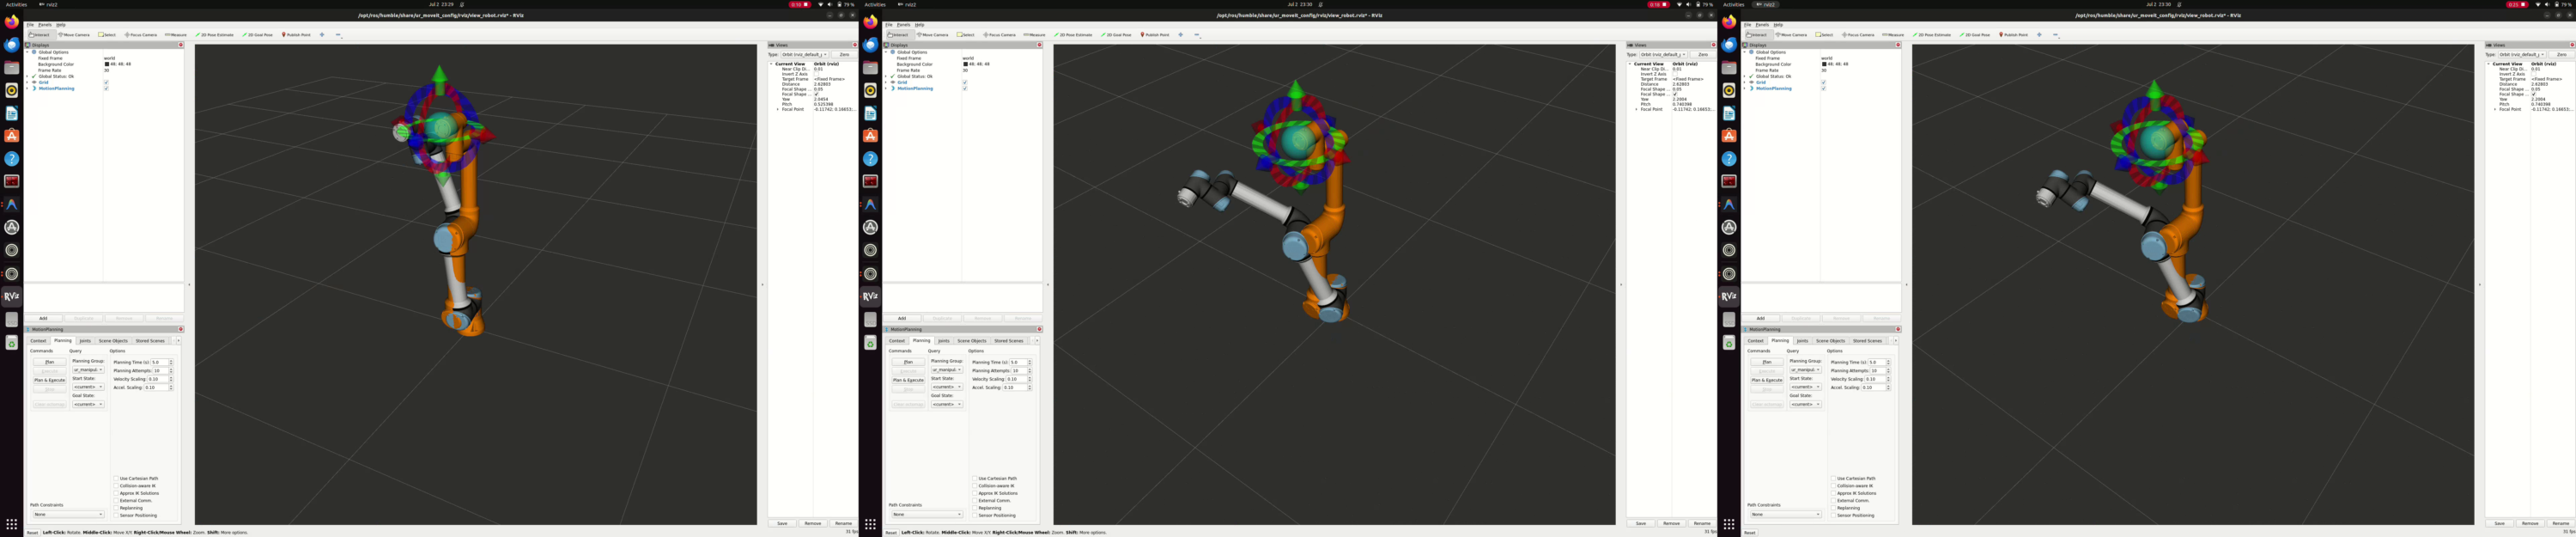
\includegraphics[width=\linewidth]{figures/ch03_trajectory_filmstrip.png}
  \caption{Frames from the screen recording of the two-waypoint trajectory executing in RViz
  --- the arm sweeping from home-ish through the elbow-bent midpoint to the target pose,
  commanded by \texttt{send\_trajectory.py} with no MoveIt in the loop.}
  \label{fig:filmstrip}
\end{figure}

\paragraph{The limit experiment: an impossible motion, executed.} Commanding the elbow to
$4.0$\,rad --- ${\sim}49^\circ$ past its $\pm\pi$ URDF limit --- produced neither a rejection
nor a clamp: \emph{the mock arm simply performed the impossible motion.} Three layers each
declined to protect us, and knowing which is which matters:
\begin{enumerate}
  \item \textbf{The trajectory controller} interpolates and forwards; Humble's JTC does not
  validate goals against URDF position limits.
  \item \textbf{Mock hardware} accepts any command --- that is what ``mock'' means.
  \item \textbf{MoveIt}, the layer that \emph{does} respect URDF limits when planning, was
  deliberately not in the loop --- our raw action client bypassed the only guard present.
\end{enumerate}
On the real UR, the vendor controller would have refused. On \emph{our} arm, there is no
vendor controller --- we are the vendor. Consequences adopted:
\begin{itemize}
  \item The Phase-1 hardware interface enforces joint limits (position, velocity, effort) in
  \texttt{read}/\texttt{write}, independent of anything upstream.
  \item The skills layer's trajectory sanity-checker (chapter's first lesson) gains a
  limits check --- names, limits, monotonic timing --- in front of \emph{every} action goal.
  \item Simulation passing is not evidence of safety when the simulation layer doesn't model
  the constraint. Know what each sim tier actually enforces (mock $<$ Isaac physics $<$
  hardware).
\end{itemize}
